% fichier clinux.tex
% sous  github.../bstarynk/misc-basile/CoursLinux
% licence CC-BY-SA
% Copyright 2025 Basile STARYNKEVITCH, 92340 Bourg-la-Reine
%
% need debian package texlive-latex-extra & texlive-bibtex-extra &
% texlive-full
% cf https://www.unilim.fr/pages_perso/stephane.vinatier/LaTeX/guide-lualatex.pdf
% cf https://fr.overleaf.com/gallery/tagged/beamer
% cf https://tex.stackexchange.com/a/527167
\documentclass[lualatex,11pt,a4paper,svgnames,french]{beamer}
%https://deic.uab.cat/~iblanes/beamer_gallery/
\usetheme{AnnArbor}
%\usepackage[T1]{fontenc}
% inputenc is not needed with lualatex
% \usepackage[utf8x]{inputenc}
\usepackage{alltt}
% https://tex.stackexchange.com/a/342804/42406
% IMPORTANT! see also: https://tex.stackexchange.com/a/500963/42406
%\usepackage{textcomp}
%\usepackage{moreverb}
%\usepackage{fancyvrb}
%\usepackage{fancyhdr}
%\usepackage{fancybox}
% https://tex.stackexchange.com/a/226497/42406
%\usepackage[title]{appendix}
% libertine, see https://tex.stackexchange.com/a/9868/42406
%\usepackage{libertine}
%\usepackage{epsfig}
%\usepackage{graphicx}
%\usepackage{float}
%\usepackage{xcolor}
%\usepackage{moreverb}
%\usepackage{multirow}
%\usepackage{boxedminipage}
%\usepackage[square]{natbib}
% https://tex.stackexchange.com/a/16992/42406
%\usepackage{mathabx}
%\usepackage{charter}
%\usepackage{inconsolata}
%\usepackage{hevea}
%\usepackage{listings}
\usepackage{relsize}
%\usepackage{verbatimbox}
%\usepackage{verbatim}
%\usepackage{filecontents}
%\usepackage{catchfile}
%\usepackage{lastpage}
%\usepackage{stmaryrd}
%\usepackage{ucs}
%\usepackage{stix}
%\usepackage{newunicodechar}
% bigfoot enables \verb in footnotes
%\usepackage{bigfoot}
%\usepackage{makeidx}
%\usepackage{times}
% https://tex.stackexchange.com/a/413066/42406
%\usepackage{apptools}
%\usepackage[a4paper, margin=2cm]{geometry}
\usepackage{hyperref}

\newcommand{\clbemail}[1]{{\href{mailto:#1}{\texttt{\textbf{\textcolor{Navy}{#1}}}}}}
\newcommand{\clburl}[1]{{\href{https://#1}{\texttt{\relsize{-1}{\textbf{#1}}}}}}
\newcommand{\clbrougras}[1]{{\textcolor{Red}{\textbf{#1}}}}
\title{Cours sur Linux} 
\author{Basile \textsc{Starynkevitch}}
\date{automne 2025}

% see also http://www.sascha-frank.com/Arrow/latex-arrows.html
% and http://tug.ctan.org/info/symbols/comprehensive/symbols-a4.pdf
% and https://ctan.math.illinois.edu/macros/latex/contrib/newunicodechar/newunicodechar.pdf
%%%% keep in order
%U+21A6 RIGHTWARDS ARROW FROM BAR
%\newunicodechar{↦}{$\mapsto$}
%U+21B3 DOWNWARDS ARROW WITH TIP RIGHTWARDS
%\newunicodechar{↳}{\rotatebox[origin=c]{180}{$\Lsh$}}
%U+2208 ELEMENT OF
%\newunicodechar{∈}{$\in$}
% U+00AB LEFT-POINTING DOUBLE ANGLE QUOTATION MARK
%\newunicodechar{«}{\guillemotleft}
% U+00BB RIGHT-POINTING DOUBLE ANGLE QUOTATION MARK
%\newunicodechar{»}{\guillemotright}
% U+00B1 PLUS-MINUS SIGN
%\newunicodechar{±}{$\pm$}
% U+00B5 MICRO SIGN
%\newunicodechar{µ}{$\mu$}

\include{gener-macro}

\begin{document}

\begin{frame}
\titlepage
\end{frame}

\begin{frame}{Un cours sur Linux}

  par

  \begin{center}Basile STARYNKEVITCH \\
  8, rue de la Faïencerie \\
  92340 Bourg-la-Reine \\
  courriel: \clbemail{basile@starynkevitch.net}
  \end{center}
  \bigskip
  
  généré: \textit{\clbdate} 

  \bigskip
  
  git: \texttt{\clbgitid}

  \begin{center}
    Ce cours contient des références
    \href{https://fr.wikipedia.org/wiki/Raisonnement_circulaireq}{\textcolor{Navy}{circulaires}}
    et des
    \href{https://fr.wikipedia.org/wiki/Hyperlien}{\textcolor{Navy}{hyperliens}}
  \end{center}
\end{frame}

\begin{frame}{Plan}
  \tableofcontents
\end{frame}

%%%%%%%%%%%%%%%%%%%%%%%%%%%%%%%%%%%%%%%%%%%%%%%%%%%%%%%%%%%%
%%%%%%%%%%%%%%%%%%%%%%%%%%%%%%%%%%%%%%%%%%%%%%%%%%%%%%%%%%%%
\section{Introduction et terminologie}
\label{sec:intro}
%%%%
\begin{frame}\frametitle{§ \ref{sec:intro}}
{\Large \clbrougras{introduction et terminologie}}
\end{frame}
%%%%
\begin{frame}\frametitle{Pourquoi j'apprécie Linux}

  \begin{itemize}
  \item Par habitude
  \item Linux est largement utilisé: des tablettes (ou
    \href{https://www.raspberrypi.org/}{RaspBerryPi}) ou
    téléphones\footnote{Android est une variante de Linux, et les
    FairPhones tournent sous une variante plus libre nommée
    \texttt{/e/OS}}, à l'affichage des gares et des bus, probablement
    dans beaucoup de voitures automobiles\footnote{Pour les fonctions
    non-critiques telles que le GPS ou la radio!}, la plupart des
    serveurs Web, aux superordinateurs\footnote{Tous les
    superordinateurs listés sur \clburl{top500.org} tournent sous
    Linux mais valent des millions d'€ et consomment parfois des MW
    électriques.}
  \item Linux est majoritairement composé de \clbrougras{logiciels libres}\footnote{Mais beaucoup
  d'entreprises vendent des logiciels propriétaires ou des services commerciaux sur
  Linux}, voir aussi \clburl{linuxfoundation.org},
    \clburl{april.org}, \clburl{aful.org}, \clburl{fsfe.org}

  \end{itemize}
  \end{frame}

%%%%
\begin{frame}\frametitle{Code source et code binaire}

Le matériel informatique\footnote{Une carte mère actuelle contient en
2025 des millions d'octets de code binaire, son ``firmware'' ou
``micrologiciel''} ne comprend que (ou ``exécute'') du \textbf{code
  binaire} ou \textbf{code machine}.

\medskip

Le dévelopeur informaticien ne comprend que du \textbf{code source}
qui est tapé au clavier\footnote{Un dévelopeur utilise aussi une
souris d'ordinateur, qui contient, comme son clavier, du code
binaire.\\} et lu à
l'écran. Empiriquement \clbrougras{un dévelopeur} à temps
plein \textbf{produit} \clbrougras{quelques dizaines de
    milliers de lignes de code source par an}.

\medskip

Dans le détail c'est très compliqué, et \textbf{il existe} des codes binaires
ou \textbf{des logiciels qui manipulent, analysent, modifient} voire
améliorent \textbf{du code source ou du code binaire}.


\medskip

Le code source est la forme préférée par le programmeur, et la plus chère.
\end{frame}

%%%%
\begin{frame}\frametitle{Variété des logiciels et des projets}
  Certains logiciels sont critiques:
  \begin{itemize}
  \item logiciel (et matériel) de pilotage d'un métro automatique
  \item logiciel d'un respirateur Covid (projet
    \href{https://github.com/Recovid/}{\textcolor{Navy}{Recovid}}).
  \end{itemize}
  D'autres le sont moins, mais on d'autres contraintes:
  \begin{itemize}
  \item logiciel de jeu  {\relsize{-1}{(doit être fini pour avant Noël)}}
  \item logiciel de comptabilité {\relsize{-1}{(doit suivre les contraintes et les normes légales)}}
  \item logiciel de bureautique (projet \clburl{libreoffice.org})
  \item logiciel
    \href{https://fr.wikipedia.org/wiki/Compilateur}{\textcolor{Navy}{\textit{compilateur}}}
    {\relsize{-1}{(traduisant le code source en binaire)}} dont \clburl{gcc.gnu.org}
    et \clburl{ocaml.org}  {\relsize{-1}{(doit suivre les usages et les standards)}}
  \item projet scolaire ou universitaire
  \end{itemize}

  
\end{frame}


%%%%
\begin{frame}\frametitle{Obligations légales et de bon sens}

  Se comporter en \href{https://fr.wikipedia.org/wiki/Bon_père_de_famille}{\textit{\textcolor{Navy}{bon père de famille}}} et en
  \href{https://fr.wikipedia.org/wiki/Proffessionnel}{\textit{\textcolor{Navy}{professionnel}}}

      \begin{itemize}
      \item en France: articles 323 et suivants du code pénal.
      \item ne pas coder volontairement des \href{https://fr.wikipedia.org/wiki/Logiciel_malveillant}{logiciels malveillants}
        \item
          \href{https://fr.wikipedia.org/wiki/Loi_de_Murphy_(homonymie)}{loi
            de Murphy}: \textbf{les catastrophes arrivent au plus mauvais moment}.
        \item \clbrougras{définir les données et les codes qui vous sont chers}.
          \item \clbrougras{sauvegarder} ceux ci
            {\relsize{-0.5}{(notamment le code source qui vous
                co-dévelopez)}} \clbrougras{périodiquement}
            {\relsize{-0.5}{(3 fois par semaine)}}, peut-être à
            distance.
            \item nettoyez préventivement plusieurs fois par ans vos
              ordinateurs {\relsize{-0.5}{(ils prennent la poussière et brûlent)}}.
      \end{itemize}

      Savoir que \textbf{tout logiciel est bogué}, donc \textbf{il
        faut \clbrougras{documenter} votre travail}.
\end{frame}

%%%%
\begin{frame}\frametitle{Architecture d'ordinateurs}

  \clbrougras{Document écrit spécifiant une famille d'ordinateurs}
  \medskip
  

  Ce document fait souvent \textbf{des milliers de pages} et donne:
  \begin{itemize}
  \item la définition des instructions machines : \clbrougras{le jeu d'instructions} ``instruction set architecture'' (ISA)
  \item le comportement de chaque instruction machine
  \item la définition de la connectique  {\relsize{-0.5}{(ports USB, HDMI, Ethernet, ...)}}
  \item souvent des spécifications électriques ou physiques
  \item parfois des spécifications temporelles; {\relsize{-0.5}{par exemple dans tel
    cas l'addition de deux entiers de 32 bits prendra 5 ns.}}
  \end{itemize}

  \bigskip
  Un ordinateur a \textbf{plusieurs sortes de mémoire}: registres,
  caches, mémoire principale (RAM), disques ou SSD.
\end{frame}

%%%%
\begin{frame}\frametitle{Architectures Von Neumann et Harvard}

  \begin{itemize}
    \item
      \href{https://fr.wikipedia.org/wiki/Architecture_de_von_Neumann}{\textcolor{Navy}{\textit{architecture
            de Von Neumann}}}: \clbrougras{les données et le code
        binaire sont dans une mémoire commune}; un logiciel pourrait
      donc modifier son propre code binaire\footnote{Certains codes
      dont le micrologiciel UEFI demeurent en mémoire ``morte'' ou à
      lecture seule.} (ou un autre).
    \item
      \href{https://fr.wikipedia.org/wiki/Architecture_de_type_Harvard}{\textcolor{Navy}{\textit{architecture
            de Harvard}}}: les données et le code mémoire ont chacun
        leur mémoire; l' auto-modification du code binaire est impossible.
  \end{itemize}

  \bigskip

  \begin{relsize}{-0.5}
  Architecture de von Neumann: tous les ordinateurs portables ou fixes sous Linux.

  \medskip
  
  Architecture Harvard: les microcontrôleurs dans les souris,
  claviers, certains contrôleurs d'écran.
  \end{relsize}
  
  \medskip

  \href{https://fr.wikipedia.org/wiki/Microarchitecture}{\textcolor{Navy}{microarchitecture}}: détails techniques sur les circuits dans un processeur
\end{frame}
%%%%
\begin{frame}\frametitle{exemple d'architecture: \clburl{riscv.org} (Von Neumann)}
  {\relsize{-1}{$\mathrm{XLEN} \in \{32, 64\}$}}   (exemples, en réalité centaines de pages)

  \smallskip


  %% cf https://tex.stackexchange.com/a/116524/42406
  \begin{tabular}{l|l}
    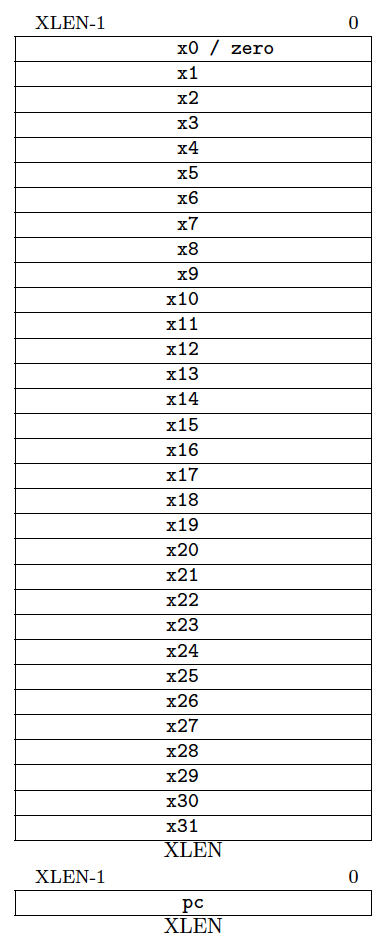
\includegraphics[scale=0.4]{base-unpriv-reg-state} &
    \raisebox{4cm}{
    \begin{tabular}{c}
      
\includegraphics[scale=0.42]{riscv-op-int} \\
      {\relsize{-1}{opération arithmétique entière sur 3 registres}} \\
      \texttt{RD := RS1 \textit{op} RS2} \\
      \hline \\
      
\includegraphics[scale=0.42]{riscv-opint-u} \\
      {\relsize{-1}{opération arithmétique entière sur constante immédiate}} \\
        \texttt{RD := RD \textit{op} IMM} \\
    \end{tabular}
      }
  \end{tabular}
\end{frame}
%%%%
\begin{frame}\frametitle{Modes noyau et utilisateur d'un processeur}


  \begin{relsize}{-0.6}
  Chaque c{\oe}ur de processeur\footnote{Selon son modèle,
  un processeur a 4 à 128 c{\oe}urs qui fonctionnent simultanément,
  chacun exécutant un code souvent différent. Je suppose ici un processeur
  \href{https://fr.wikipedia.org/wiki/X64}{\textcolor{Navy}{\textit{x86-64}}} ...\\} fonctionne dans l'un des deux modes suivants:
  \begin{itemize}
    \item le \textbf{mode noyau} (ou privilégié) permet l'exécution de
      toutes les instructions machine, y compris les plus dangereuses
      qui écrivent sur les disques, affichent à l'écran, ou éteignent
      l'ordinateur. Seul le noyau Linux (et UEFI) utilise ce mode.

      \item le \textbf{mode utilisateur} interdit les instructions machine
        dangereuses, mais permet les operations sûres (addition
        entière, accès contrôlé à \textit{certaines} zones
        mémoire). Le code binaire dans les segments des fichiers
        exécutables s'exécute fan ce mode.
  \end{itemize}
  
  Une instruction machine particulière \texttt{SYSCALL}\footnote{Je
  simplifie, il y en a plusieurs!} permet de passer du mode utilisateur
  au mode noyau. Une autre \texttt{SYSRETURN} passe de manière
  contrôlée du mode noyau au mode utilisateur.
  \end{relsize}
\end{frame}
%%%%
\begin{frame}\frametitle{les interruptions}

  Tout processeur accepte des  \href{https://fr.wikipedia.org/wiki/Interruption_(informatique)}{\textcolor{Navy}{interruptions}} sur des évènements tels que :

  \begin{relsize}{-0.5}
  \begin{itemize}
  \item instruction machine interdite ou inexistante
  \item évènement ou incident matériel 
  \item réception ou fin d'émission d'un paquet de données (vers un
    disque, un port USB ou Ethernet)
  \item temporisation atteinte
  \item adresse de donnée ou de code illicite
  \item division par 0
  \end{itemize}
  \end{relsize}
  
  Le processeur sauvegarde alors son état\footnote{L'état sauvegardé par le
  matériel peut être partiel, à charge pour le code du noyau de
  sauvegarder explicitement le reste de l'état} et passe le contrôle à
  du code machine spécifique en mode noyau.
\end{frame}

%%%%
\begin{frame}\frametitle{rôles du noyau Linux}

  \begin{itemize}
  \item gérer et abstraire le matériel spécifique
  \item offrir aux logiciels applicatifs\footnote{Les applications et
  logiciels serveurs Linux tournent en mode utilisateur et utilisent
  le noyau Linux par des appels systèmes} via les appels systèmes une
    abstraction de plus haut niveau:
    \begin{itemize}
    \item les fichiers
    \item les protocoles réseaux (TCP)
    \item les processus
    \end{itemize}
    \item cette interface normalisée permet la portabilité du code
      source (quand le dévelopeur y travaille) et dans des cas
      particulier de certains fichiers binaires exécutables.
    \item Linux est
      \href{https://fr.wikipedia.org/wiki/Multitâche}{\textbf{\textcolor{Navy}{multitâches}}}
      et \href{https://fr.wikipedia.org/wiki/Multi-utilisateur}{\textbf{\textcolor{Navy}{multi-utilisateurs}}}
      \item Conformité aux normes \href{https://fr.wikipedia.org/wiki/POSIX}{\textbf{\textcolor{Navy}{POSIX}}}  et \href{https://fr.wikipedia.org/wiki/Single_UNIX_Specification}{\textbf{\textcolor{Navy}{Single UNIX specification}}}
  \end{itemize}
\end{frame}


%%%%
\begin{frame}\frametitle{espace d'adressage et mémoire virtuelle}
  \begin{tabular}{l|p{5cm}}
    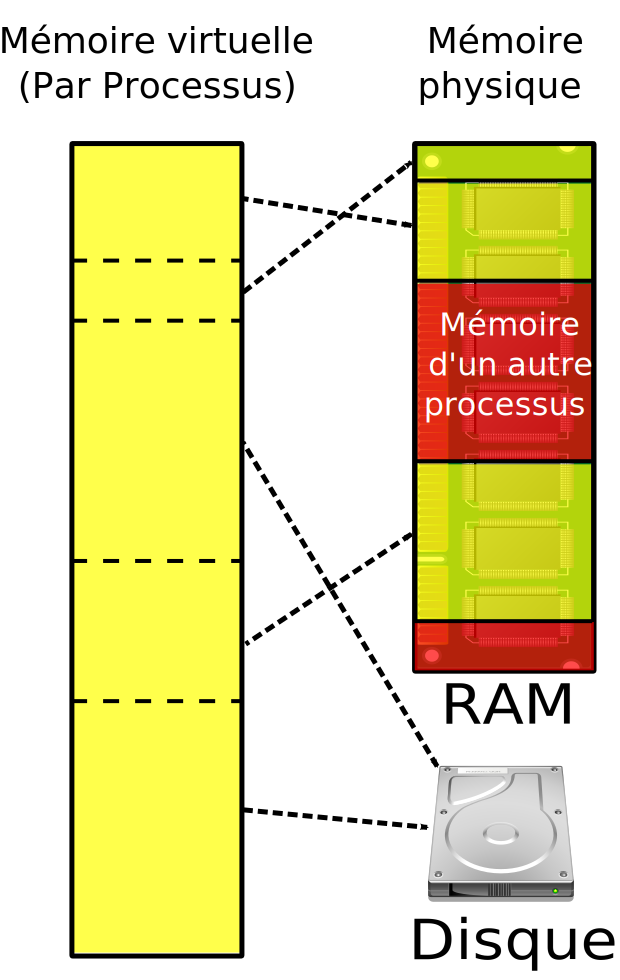
\includegraphics[height=0.6\textheight]{memoire-virtuelle-wikip}
    &
    \raisebox{3.5cm}{
      \parbox{5cm}{ Le noyau gère des segments\footnote{Il y a des milliers de segments pour des centaines de processus. Certaines pages de ces segments sont chargés à la demande (sur interruption) par le noyau.\medskip\\} de mémoire (code,
        données) dont certains sont en lecture seule et d'autres
        seulement sur le disque. Ces segments sont des multiples de
        pages {\relsize{-1}{(4Ko ou 1Mo)}}.
    }}
  \end{tabular}
\end{frame}

%%%%
\begin{frame}\frametitle{distributions Linux}

  Elles contiennent un grand nombre de \textcolor{red}{\textbf{paquets\footnote{plusieurs milliers de
  paquets; il est souhaitable, une fois que vous maitrisez Linux dans
  un cadre professionnel, d'y contribuer, en installant un
  serveur de paquet d'une distribution sur le serveur qui vous sera
  affecté.\\} logiciels}}. Sur une
  clef USB (ou des CDROMs) on trouve de quoi installer Linux sur un
  ordinateur connecté à Internet. L'installation prend quelques heures
  et va télécharger d'autres paquets depuis un serveur distant.

  \medskip
  
  Beaucoup de
  \href{https://fr.wikipedia.org/wiki/Distribution_Linux}{\textcolor{Navy}{\textit{distributions}}}
  GNU/Linux sont facilement téléchargeables et redistribuables:
    \begin{itemize}
    \item \textbf{Debian} sur \clburl{debian.org}
    \item \textbf{Ubuntu} sur \clburl{ubuntu.com}, dérivée de Debian,
      et sa variante
      \href{https://fr.wikipedia.org/wiki/GendBuntu}{\textcolor{Navy}{GEndBuntu}}
    \item \textbf{Mageia} sur \clburl{mageia.org}
    \item \textbf{RedHat} sur \clburl{redhat.com}
    \end{itemize}
\end{frame}
%%%%
\begin{frame}\frametitle{Variété des distributions}

Il existe des distributions non linuxiennes mais plus ou moins libres:
\clburl{freebsd.org}, \clburl{openbsd.org}, \clburl{hurd.gnu.org},
\clburl{tunes.org}, \href{https://sources.vsta.org:7100/}{VSTa},
\clburl{templeos.org}, \clburl{illumos.org} etc...

\medskip

Dans le monde des distributions Linux on peut distinguer:

\begin{relsize}{-0.6}
\begin{itemize}
\item les \textbf{distributions \textcolor{red}{binaires}}
  (\clburl{ubuntu.com} comme \clburl{linuxmint.com} et beaucoup
  d'autres, souvent dérivées de \clburl{debian.org}, et
  \clburl{redhat.com}) qui existent sous plusieurs versions de
  stabilité et nouveauté variées. Elles sont recommandées pour les
  débutants (ou ceux sont pressés d'avoir un ordinateur utilisable
  sous Linux). Plusieurs distributions facilitent\footnote{En
  pratique, à chaque redémarrage, on choisit au clavier quel système
  va démarrer.\medskip} la cohabitation sur un ordinateur de Linux
  avec Windows.

\item les \textbf{distributions \textcolor{red}{sources}}
  (\clburl{gentoo.org} et \clburl{archlinux.org} parmi d'autres) qui
  compilent les paquets logiciels à leur installation. Elles
  s'adressent à des experts, et leur installation prendra du temps
  mais peut être optimale.
\end{itemize}
\end{relsize}
\end{frame}



%%%%
\begin{frame}\frametitle{Libertés du logiciel libre}

Elles sont définies dans différentes licences logicielles,
principalement La
\href{https://fr.wikipedia.org/wiki/Licence_publique_générale_GNU}{licence
  publique GNU} GPL
\href{https://www.gnu.org/licenses/gpl-3.0.html}{3.0} (en
\clburl{www.gnu.org/licenses/}), la licence LGPL, les licences
\clburl{cecill.info} ou \clburl{eupl.eu}, et d'autres.

La GPL est ma licence logicielle préférée, et permet:
\begin{itemize}
\item {\relsize{-1}{(liberté 0)}} la \textbf{\textcolor{red}{liberté
    d'exécuter}} le logiciel pour n'importe quel usage;
\item {\relsize{-1}{(liberté 1)}} la  \textbf{\textcolor{red}{liberté d'étudier le
  fonctionnement}} d'un programme et de l'adapter à ses besoins, ce qui
  passe par l'accès aux codes sources;
\item {\relsize{-1}{(liberté 2)}} la  \textbf{\textcolor{red}{liberté de redistribuer}} des
  copies du logiciel;
\item {\relsize{-1}{(liberté 3)}} \textbf{\textcolor{red}{la liberté de faire
  bénéficier\footnote{Il y a alors l'obligation morale voire légale de
  redistribuer le code source du logiciel amélioré sous la même
  licence, c'est le
  \href{https://fr.wikipedia.org/wiki/Copyleft}{\textcolor{red}{copyleft}}!} la
  communauté}} des versions modifiées.
\end{itemize}

\smallskip

\begin{relsize}{-1}
  Un logiciel propriétaire a sa licence et ses obligations légales. Sa
  redistribution est souvent interdite, son exécution, sa
  modification, son analyse est limitée par contrat.
\end{relsize}
\end{frame}

%%%%
\begin{frame}\frametitle{Économie du logiciel libre}
Ils ne sont \textbf{pas gratuits}

\medskip

C'est un
\href{https://fr.wikipedia.org/wiki/Bien_commun}{\textcolor{Navy}{bien
    commun}} (cf livres et publications de
\href{https://fr.wikipedia.org/wiki/Jean_Tirole}{\textcolor{Navy}{Jean
    Tirole}}).

\medskip

La difficulté est d'organiser et de faire vivre une \href{https://fr.wikipedia.org/wiki/Communauté_du_logiciel_libre}{\textcolor{Navy}{communauté}}. 

\medskip

Il peut exister des financements institutionnels
\href{https://fr.wikipedia.org/wiki/Horizon_Europe}{\textcolor{Navy}{Horizon
    Europe}} ou
\href{https://fr.wikipedia.org/wiki/Agence_nationale_de_la_recherchee}{\textcolor{Navy}{ANR}}
ou \clburl{itea4.org} et il faut les favoriser

\medskip

Voir le moteur d'inférences libre
\href{https://github.com/RefPerSys/RefPerSys/}{\textcolor{Navy}{RefPerSys}}
(``reflexive persistent system'') et les livres (et logiciels) de
\href{https://fr.wikipedia.org/wiki/Jacques_Pitrat}{\textcolor{Navy}{Jacques
    Pitrat}}

\smallskip
  La
  \href{https://fr.wikipedia.org/wiki/Souveraineté_numérique}{\textit{\textcolor{Navy}{souveraineté
        numérique}}} est un argument pour le développement, le
  financement, et l'amélioration de logiciels libres...
\end{frame}


%%%%%%%%%%%%%%%%%%%%%%%%%%%%%%%%%%%%%%%%%%%%%%%%%%%%%%%%%%%%%%%%
%%%%%%%%%%%%%%%%%%%%%%%%%%%%%%%%%%%%%%%%%%%%%%%%%%%%%%%%%%%%%%%%
\section{Démarrage d'un système Linux} % How Linux starts
\label{sec:start-linux}
%%%%
%%%%
\begin{frame}\frametitle{§ \ref{sec:start-linux}}
{\Large \clbrougras{Démarrage d'un système Linux}}
\end{frame}
%%%
\begin{frame}\frametitle{Démarrage d'un système Linux déjà installé}

  Comment démarre à froid un ordinateur Linux\footnote{Le démarrage
  rarissime d'un supercalculateur est très complexe et je ne pourrais
  pas l'expliquer en détail.} (portable ou fixe), où une distribution
  Linux a déjà été installée il y a plusieurs mois.

  \begin{relsize}{-0.5}
  \begin{enumerate}
  \item le micrologiciel
    (de nos jours,
    \href{https://fr.wikipedia.org/wiki/UEFI}{\textcolor{Navy}{\textit{UEFI}}}
    et autrefois le BIOS)
    de la carte mère démarre et initialise le matériel. Une
    \href{https://fr.wikipedia.org/wiki/Mémoire_flash}{\textcolor{Navy}{mémoire
        flash}} contient le paramétrage pour ça.
    \item un chargeur (``boot-loader'', un code binaire de quelques kilo-octets) est
      chargé dans la mémoire vive; c'est le logiciel libre \clburl{www.gnu.org/software/grub} codé en assembleur et C.
      \item ce logiciel chargeur met en mémoire plusieurs zones (ou
        ``fichiers''?) de code binaire, dont le
        \href{https://fr.wikipedia.org/wiki/Noyau_Linux}{\textcolor{Navy}{noyau Linux}} et plusieurs modules
        \href{https://fr.wikipedia.org/wiki/Linux_Security_Module}{\textcolor{Navy}{de sécurité}}
     \item le noyau peut démarrer le processus initial dont le binaire
       est dans le fichier \texttt{/sbin/init}
  \end{enumerate}
  \end{relsize}
\end{frame}

%%%%
\begin{frame}\frametitle{Fichiers, processus, appels système (notions)}
  %

  \begin{relsize}{-0.5}
Un \textbf{\textcolor{red}{fichier}} (``file'') générique (Linux) est
\textbf{\textcolor{red}{une séquence d'octets} avec des méta-données}
la décrivant. Il existe plusieurs sortes de fichiers\footnote{La
majorité des fichiers demeurent sur le[s] disque[s] de l'ordinateur
même quand il est éteint, mais il y a des exceptions!} : certains sont
des répertoires faisant référence à d'autres fichiers, d'autres sont
des liens symboliques pointant par un nom vers un fichiers, et
d'autres (soquettes) permettent la communication entre
processus. Certains fichiers contiennent du code binaire exécutable
organisés en segments.

\medskip

Un \textbf{\textcolor{red}{processus}} (``process'') Linux
\textbf{\textcolor{red}{est un programme en train de s'exécuter}}. Le
noyau gère les fichiers nécessaires à l'exécution de ce programme. Un
ordinateur éteint n'a pas de processus.

\medskip

Un \textbf{\textcolor{red}{appel système}} (``system call'') est une
opération ``atomique'' exécutée par un processus dans le code binaire
d'un fichier programme qui est exécutée par le noyau. La plupart des
\href{https://fr.wikipedia.org/wiki/Appel_système}{\textcolor{Navy}{appels
    systèmes}} s'exécutent en quelques dizaines de µs. Il y a environ
380 appels systèmes possibles (cf \href{https://man7.org/linux/man-pages/man2/syscalls.2.html}{\textcolor{Navy}{\texttt{syscalls(2)}}}).
\smallskip
  \end{relsize}
\end{frame}

%%%%
\begin{frame}\frametitle{protocole et exemple d'appel système}
  Un appel système transmet entre 0 et 7 arguments fixes \footnote{Un
  argument d'un appel système est un entier ou un pointeur vers une
  donnée de l'espace d'adressage du processus faisant l'appel.\\} passés
  dans des registres. Il peut échouer.

  Exemple:
  \href{https://man7.org/linux/man-pages/man2/munmap.2.html}{\textcolor{Navy}{\texttt{munmap(2)}}}
  pour ôter un segment dans l'espace d'adressage du processus courant.

  \begin{quote}
  \begin{alltt}
    void* ad = \clbrougras{\textrm{\textit{une adresse}}};\\
    size\_t sz = \clbrougras{\textrm{\textit{une longueur}}};\\
    int ech = munmap(ad, sz);
  \end{alltt}
  \end{quote}
  
  \smallskip
  
  Si l'appel échoue, \texttt{ech} vaut -1 et
  \href{https://man7.org/linux/man-pages/man3/errno.3.html}{\textcolor{Navy}{\texttt{errno(3)}}}
  contient un code d'erreur\footnote{Ici ça pourrait être
  \texttt{EINVAL} donc 22 (argument incorrect, par exemple si
  \texttt{ad} n'est pas aligné à une page) ou \texttt{EINTR} donc 4 si
  l'appel système a été interrompu.\medskip\\}.

  \smallskip
\end{frame}

%%%%%%%%%%%%%%%%%%%%%%%%%%%%%%%%%%%%%%%%%%%%%%%%%%%%%%%%%%%%
%%%%%%%%%%%%%%%%%%%%%%%%%%%%%%%%%%%%%%%%%%%%%%%%%%%%%%%%%%%%
\section{processus Linux}
\label{sec:process}
%%%%
\begin{frame}\frametitle{§ \ref{sec:process}}
{\Large \clbrougras{processus dans Linux}}
\end{frame}
%%%%%%%%%

\begin{frame}\frametitle{Le processus initial}
  \clbrougras{C'est le seul processus qui n'est pas démarré par un
    autre processus}, mais par le noyau\footnote{On peut paramétrer le
  chargeur GRUB pour que le noyau démarre avec un autre processus
  initial.\\ Certains systèmes Linux faisaient démarrer par le noyau
  certains processus sur des évènements extérieurs, par exemple
  l'insertion d'une clef USB.\\} au démarrage de Linux.

  \bigskip
  
  \clbrougras{Ce processus initial} (executable \texttt{/sbin/init} ou
  \href{https://fr.wikipedia.org/wiki/Systemd}{\textcolor{Navy}{systemd}})
  \clbrougras{ne doit pas s'arrêter} (sauf arrêt de l'ordinateur) donc
  a des contraintes et propriétés particulières.

  \bigskip

  Chaque processus a un
  \href{https://fr.wikipedia.org/wiki/Identifiant_de_processus}{\textcolor{Navy}{numéro
      identifiant}} \clbrougras{unique}, son \texttt{\textit{pid\_t}} (cf
  \href{https://man7.org/linux/man-pages/man2/getpid.2.html}{\textcolor{Navy}{\texttt{getpid(2)}}}). Celui
  du processus initial est 1.
\end{frame}
%%%%
\begin{frame}\frametitle{Gestion des processus par le noyau}
  \begin{relsize}{-0.5}
  Tous les processus sont gérés (et connus) par le noyau et
  beaucoup\footnote{Il y a plusieurs centaines de processus, mais la
  plupart attendent un événement extérieur. Voir
  \href{https://man7.org/linux/man-pages/man2/poll.2.html}{\texttt{\textcolor{Navy}{poll(2)}}}
  et
  \href{https://man7.org/linux/man-pages/man2/wait.2.html}{\texttt{\textcolor{Navy}{wait(2)}}}. Un
  ordinateur portable peut avoir 1 ou 2 processus actifs et 300
  inactifs.}  sont inactifs. Le noyau connait et modifie
  périodiquement le processus courant sur chaque c{\oe}ur de
  processeur, et gère pour chaque processus (cf 
  \href{https://man7.org/linux/man-pages/man7/credentials.7.html}{\texttt{\textcolor{Navy}{credentials(7)}}}):
  \end{relsize}

  \begin{relsize}{-1}
  \begin{itemize}
  \item l'espace d'adressage, le \textit{pid} et celui du père
    \href{https://man7.org/linux/man-pages/man2/getppid.2.html}{\texttt{\textcolor{Navy}{getppid(2)}}}
    \item les filaments ou 
      ``{\href{https://fr.wikipedia.org/wiki/Thread_(informatique)}{\textit{\textcolor{Navy}{thread}}s}}''
    \item les
      {\href{https://fr.wikipedia.org/wiki/Pile_d'exécution}{\textit{\textcolor{Navy}{pile
              d'exécution}}}} ou ``call stack''
  \item la table des
    \href{https://fr.wikipedia.org/wiki/Descripteur_de_fichier}{\textcolor{Navy}{descripteurs
        de fichiers}} (``file descriptors'') ouverts (entiers)
  \item des limites de resources (taille maximale de fichier, de l'espace d'adressage, etc... cf
    \href{https://man7.org/linux/man-pages/man2/getrlimit.2.html}{\texttt{\textcolor{Navy}{getrlimit(2)}}})
    \item les 
    \href{https://fr.wikipedia.org/wiki/Répertoire_(informatique)}{\textcolor{Navy}{\textit{répertoires}}} courant (cf
    \href{https://man7.org/linux/man-pages/man2/getcwd.2.html}{\texttt{\textcolor{Navy}{getcwd(2)}}}) et racine (cf
    \href{https://man7.org/linux/man-pages/man2/chroot.2.html}{\texttt{\textcolor{Navy}{chroot(2)}}}).
    \item les \href{https://fr.wikipedia.org/wiki/Signal_(informatique)}{\textcolor{Navy}{\textit{signaux}}} (cf
      \href{https://man7.org/linux/man-pages/man2/sigaction.2.html}{\texttt{\textcolor{Navy}{sigaction(2)}}}
      et
      \href{https://man7.org/linux/man-pages/man7/signal.7.html}{\texttt{\textcolor{Navy}{signal(7)}}}
      )
  \end{itemize}
  \end{relsize}
\end{frame}
%%%%
\begin{frame}\frametitle{Création d'un processus}
  Tout
  {\href{https://largo.lip6.fr/~cassagnea/docs/epu/main3_sys/cm/cm4-processus.pdf}{\textcolor{Navy}{\textit{processus}}}}
  non initial est le plus souvent créé par
  {\href{https://man7.org/linux/man-pages/man2/fork.2.html}{\texttt{\textcolor{Navy}{fork(2)}}}}
  et plus rarement par
  {\href{https://man7.org/linux/man-pages/man2/clone.2.html}{\texttt{\textcolor{Navy}{clone(2)}}}}
  \footnote{En pratique, l'appel système \texttt{clone} est
  principalement utilisé pour créer des filaments, donc pour réaliser
  \href{https://man7.org/linux/man-pages/man3/pthread_create.3.html}{\texttt{\textcolor{Navy}{pthread\_create(3)}}}.
  Les appels système \texttt{fork} et \texttt{clone} peuvent échouer et sont lourds et lents (millisecondes).\smallskip\\}.
  Pour \clbrougras{dupliquer le processus courant}:
  \begin{quote}
    \begin{alltt}
      pid\_t np = fork();
    \end{alltt}
  \end{quote}
  Après quoi  \clbrougras{on a deux processus quasi-identiques} qui tournent \textbf{simultanément}, sauf:
  \begin{relsize}{-1}
  \begin{itemize}
  \item dans le processus appelant (le \clbrougras{père}) \texttt{np} est non-nul
  \item dans le processus créé (le \clbrougras{fils}) \texttt{np} est
    nul, et \textbf{il a un seul filament d'exécution}.
  \end{itemize}
  \end{relsize}
  Ordinairement le fils fait des traitements courts\footnote{Par exemple, il ferme par
  {\href{https://man7.org/linux/man-pages/man2/close.2.html}{\texttt{\textcolor{Navy}{close(2)}}}}
  les descripteurs de fichiers inutiles.\medskip\\} puis démarre avec
  {\href{https://man7.org/linux/man-pages/man2/execve.2.html}{\texttt{\textcolor{Navy}{execve(2)}}}}
  un nouveau programme exécutable. Le père va plus tard attendre avec
  {\href{https://man7.org/linux/man-pages/man2/waitpid.2.html}{\texttt{\textcolor{Navy}{waitpid(2)}}}}
  la terminaison du processus fils.
\end{frame}
%%%%%%%%%%%%%%%%%%%%%%%%%%%%%%%%%%%%%%%%%%%%%%%%%%%%%%%%%%%%
%%%%%%%%%%%%%%%%%%%%%%%%%%%%%%%%%%%%%%%%%%%%%%%%%%%%%%%%%%%%
\section{fichiers sur Linux}
\label{sec:file}
%%%%
\begin{frame}\frametitle{§ \ref{sec:file}}
{\Large \clbrougras{fichiers sur Linux}}
\end{frame}

%%%%%%%%%%%%%%%%%%%%%%%%%%%%%%%%%%%%%%%%%%%%%%%%%%%%%%%%%%%%
%%%%%%%%%%%%%%%%%%%%%%%%%%%%%%%%%%%%%%%%%%%%%%%%%%%%%%%%%%%%
\section{commandes sur Linux}
\label{sec:commands}
%%%%
\begin{frame}\frametitle{§ \ref{sec:commands}}
{\Large \clbrougras{commandes sur Linux}}
\end{frame}

%%%%%%%%%%%%%%%%%%%%%%%%%%%%%%%%%%%%%%%%%%%%%%%%%%%%%%%%%%%%
%%%%%%%%%%%%%%%%%%%%%%%%%%%%%%%%%%%%%%%%%%%%%%%%%%%%%%%%%%%%
\section{bibliothèques et développement sur Linux}
\label{sec:libr-devel}
%%%%
\begin{frame}\frametitle{§ \ref{sec:libr-devel}}
{\Large \clbrougras{bibliothèques et développement sur Linux}}
\end{frame}

\end{document}
